\documentclass[12pt, oneside]{article}
\usepackage{geometry}
\usepackage[utf8]{inputenc}
\usepackage{setspace}
\usepackage{times}
\usepackage{url}
\urlstyle{same}
\usepackage{multirow}
\usepackage[usegeometry]{typearea}
% Useful for checking layout
% \usepackage{showframe}
\usepackage{fancyhdr}
\usepackage{blindtext}
% Indenting the first sentence after section
\usepackage{indentfirst}
% Set language
\usepackage[german]{babel}
% Abbreviations
\usepackage{glossaries}
% For big tables which span multiple pages
\usepackage{longtable}
% Images
\usepackage{graphicx}
\graphicspath{ {./images/} }
% APA Citation Style
\usepackage[natbibapa]{apacite}

\geometry{
 a4paper,
 left=30mm,
 top=25mm,
 right=25mm,
 bottom=20mm,
 footskip=15pt,
}

\setstretch{1.3} % Define Line Spacing
\renewcommand{\headrulewidth}{0pt} % Remove footer line

\pagestyle{fancy} % Allow for customizing header and footer
% Customize footer for page number location
\fancyhf{}
\fancyfoot{}
\fancyhead[R]{Yannick Hutter}
\fancyhead[L]{Exposé}
\fancyfoot[R]{\thepage}



 \makeglossaries

 \newglossaryentry{covid19}
 {
     name=Covid-19,
     description={Coronavirus-Krankheit-2019 ~\citep{covid19}}
 }
 \newglossaryentry{foph}
 {
     name=FOPH,
     description={Federal Office of Public Health}
 }
 \newglossaryentry{bfs}
 {
     name=BFS,
     description={Bundesamt für Statistik}
 }
 \newglossaryentry{who}
 {
     name=WHO,
     description={World Health Organization}
 }
 \newglossaryentry{crisis_visualization}
 {
     name=Crisis Visualization,
     description={Visuelle Repräsentation von Informationen über unerwünschte Situationen, welche eine Bedrohung für die Menschheit darstellen. \citep[S. 2]{mapping_landscape_of_covid19_crisis_visualizations}}
 }






\begin{document}
\pagenumbering{roman}
\begin{titlepage}
	\begin{center}
		\Huge
		\textbf{Exposé}
		
		\vspace{0.5cm}
		\LARGE
		Implementierung eines personalisierbaren COVID19 Dashboards - Erstellung und Validierung eines High Fidelity Prototyps anhand des User Centered Design Ansatzes
		
		\vspace{1.5cm}
		\normalsize
		\textbf{Yannick Hutter}\\
		\textbf{yannick.hutter@stud.fhgr.ch}
		
		\vfill
		Referrent: Daniel Klinkhammer\\
		Korefferent: Michael Burch\\
		
		\vspace{0.8cm}
		
		
		Digital Business Management\\
		Fachhochschule Graubünden\\
		April 2022
	\end{center}
\end{titlepage}



\tableofcontents
\listoffigures
\listoftables



\clearpage
\pagenumbering{arabic}
\setcounter{page}{2}

\section{Einleitung}
Die Coronavirus-Pandemie (fortlaufend als \Gls{covid19} bezeichnet) hat in grossen Teilen der Welt seine Spuren hinterlassen. So geht gemäss dem \Gls{foph} hervor, dass im Zeitraum vom 24.02.2020 bis zum 10.03.2022 mehr als 3 Millionen Ansteckungen in der Schweiz, sowie im Liechtenstein verzeichnet worden sind~\citep{covid19_laboratory_confirmed_cases}. Ein wichtiges Mittel zur Kommunikation mit der Bevölkerung sind hierbei Datenvisualisierungen, insbesondere Dashboards.

Der Begriff Dashboard kommt ursprünglich aus dem Englischen und bezieht sich auf das Armaturenbrett beim Auto, wo alle relevanten Informationen übersichtlich auf einen Blick erkenntlich sind ~\citep{dashboard_term_definition}.

Auch bei \Gls{covid19} wurden eine Vielzahl von Dashboard Visualisierungen erstellt, auf denen die wichtigsten Indikatoren der Pandemie wie Fallzahlen etc. ersichtlich sind. Ein Vertreter dieser Kateogrie wurde von der \Gls{who} erstellt und trägt die passende Bezeichnung WHO Coronavirus Dashboard ~\citep{who_dashboard}. Das eine weltweite Organisation wie WHO sich um die Erstellung von Datenvisualisierungen zur Corona Thematik bemüht, soll aufzeigen wie wichtig Dashboard-Visualisierungen geworden sind.






\clearpage
\section{Forschungsfrage}
Die Landschaft der Corona Datenvisualisierungen ist sehr breit gestrickt und umfasst underschiedlichste Repräsentanten von Visualisierungsarten. Nebst den einzelnen Visualisierungen werden diese aber auch in Form eines Dashboards zusammengefasst. Eine grosse Anzahl dieser Dashboards sind jedoch sehr allgemein gehalten und zielen auf die breite Öffentlichkeit oder Datenanalysten als Zielgruppe ab. Interessant in diesem Kontext wäre es jedoch zu untersuchen, wie sich eine spezifische Nutzergruppe solches Dashboard vorstellen würden und was für Informationen in diesem Zusammenhang relevant sind. Die Forschungsfrage lautet daher:

``Wie stellen sich Studierende an der FHGR ein personalisierbares Covid-19 Dashboard vor und wie wird dieses verwendet - Erstellung eines High Fidelity Prototypen anhand des User Centered Design Ansatzes``

\clearpage
\section{Methodische Vorgehensweise}
\subsection{Methodik}
Um die vorhergehende Forschungsfrage zu beantworten, wurde ein qualitatives Vorgehen basierend auf dem User-centered Design Prozess gewählt (siehe Abbildung 2).

\begin{figure}[ht]
	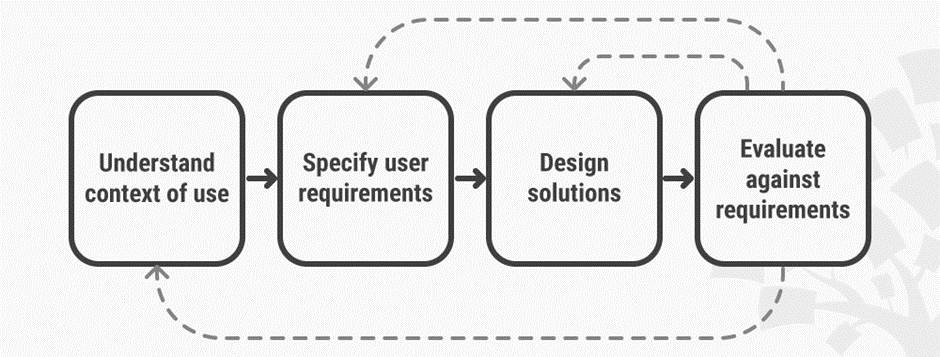
\includegraphics[width=12cm]{user-centered-design-molde.png}
	\centering
	\caption{User-centered Design Model ~\citep{public_media_user_centered_design}}
\end{figure}


Da sich die Forschungsfrage an die Zielgruppe von FHGR Studierenden richtet, wird in einem ersten Schritt deren Bedürfnisse evaluiert. Hierzu gibt es bereits Studien, welche die Erstellung von Dashboards spezielle für Software Entwickler behandeln ~\citep{design_and_validation_of_precooked_developer_dashboard}. Die Studie hat zuerst qualitative Interviews mit Software Entwicklern durchgeführt, um an die relevanten Informationen und Nutzungsszenarien zu gelangen. Um den Kontext und die Nutzeranforderungen zu evaluieren würde ich in einem ersten Schritt ebenfalls qualitative Interviews mit FHGR Studierenden durchführen.

Mit den gewonnen Erkenntnissen geht es anschliessend um die eigentliche Erstellung eines High Fidelity Prototypen. Eine weitere Studie hat bereits die Landschaft von Web basierten Corona Dashboards untersucht und verschiedene Kernpunkte definiert, welche beim erstellen dieser Dashboards von hoher Relevanz sind ~\citep{web_based_covid_dashboards}.

Für die Evaluation des erstellten Prototypen wird zum Schluss ein Aufgaben basiertes User Testing durchgeführt. Die Aufgaben basieren auf den gewonnen Erkenntissen mithilfe der im Vorfeld durchgeführten Interviews.

\clearpage
\subsection{Aufbau}
Nebst den geforderten Inhalten gemäss dem wissenschaftlichen Leitfaden wie Titelblatt, Abstract, Einleitung etc. wird die Arbeit an Hand des User-centered Design Prozesses aufgebaut und beinhaltet folgende Struktur:

\textbf{Die Landschaft der Corona Dashboards}
\begin{itemize}
	\item Dashboard - Alles auf einem Blick
	\item Von den Daten zur Visualisierung
	\item Überblick über bestehende Corona Dashboards
\end{itemize}

\textbf{Verstehen der Zielgruppe}
\begin{itemize}
	\item Definition der Zielgruppe
	\item Erhebung der Nutzeranforderungen durch qualitative Interviews
\end{itemize}

\textbf{Prototyping}
\begin{itemize}
	\item Prototyping Methoden
	\item Umsetzung High Fidelity Prototyp
\end{itemize}


\textbf{Evaluation}
\begin{itemize}
	\item Aufgaben basiertes User Testing
\end{itemize}


\textbf{Ergebnisteil}
\begin{itemize}
	\item Auswertung
	\item Interpretation der Resultate
\end{itemize}

\textbf{Diskussionsteil}
\begin{itemize}
	\item Ausblick
	\item Kritische Reflexion
	\item Limitationen der Arbeit
\end{itemize}

\clearpage
\section{Stand der Forschung}
Die Coronavirus-Pandemie greift seit ihrem Aufkommen im Jahr 2020 in eine Vielzahl von Lebensbereichen ein. Es ist wenig verwunderlich dass zu einem solch einschneidendem Thema eine grosse Anzahl von wissenschaftlichen Publikationen erstellt worden sind. Eine Publikation untersuchte die Vielzahl von Corona Datenvisualisierungen und weist ihnen verschiedene Arten von Intentionen (Aussage über den Verlauf der Pandemie etc.) zu ~\citep{mapping_landscape_of_covid19_crisis_visualizations}. Weitere Quellen untersuchten speziell für das Web zugeschnittene Corona Dashboards und leiteten daraus Design Guidelines ab ~\citep{web_based_covid_dashboards}. Andere Studien wiederum haben sich mit der Erstellung von Dashboards für spezielle Nutzergruppen auseinandergesetzt ~\citep{design_and_validation_of_precooked_developer_dashboard}. Auch wurde bereits im Zuge einer Studie die Schwierigkeiten bei der Erstellung von Corona Dashboards evaluiert ~\citep{experience_dashboard_teams_during_pandemic}

Jedoch scheint es zum jetzigen Zeitpunkt noch keine Studie zu geben, welche die Erstellung von Corona Dashboards für eine bestimmmte Zielgruppe unter Berücksichtigung eines User-centered Design Ansatzes behandelt. 

\clearpage
\section*{Anhang}
\subsection*{Rechercheprotokoll}

\begin{table}[h]
	\begin{center}
		\begin{tabular}{ |c|c|c| }
			\hline
			\textbf{Quelle}& \textbf{Schlüsselwörter}& \textbf{Relevante Artikel}\\
			\hline
			\multirow{3}{*}{https://scholar.google.com/}&\multirow{3}{3cm}{data visualization covid 19}& ~\citep{data_visualization_for_understanding_of_covid19}\\
			  &   & ~\citep{big_data_visualization_and_visual_analytics_of_covid_19_data} \\&& ~\citep{mapping_landscape_of_covid19_crisis_visualizations}\\
			\hline
			\multirow{2}{*}{https://scholar.google.com/} & \multirow{2}{4cm}{key factors for
			simple data visualization}&~\citep{datenvisualisierungen_grundlagen_und_praxis}\\&& ~\citep{datenvisualisierungen_modern_web}\\
			\hline
		\end{tabular}
		\caption{\label{tab:research-protocol}Rechercheprotokoll (Eigene Darstellung)}
	\end{center}
\end{table}

\subsection*{Zeitplan}

\begin{table}[h]
	\begin{center}
		\begin{tabular}{ |c|c| }
			\hline
			\textbf{Tätigkeit}& \textbf{Stichtag}\\
			\hline
			Verbesserung Exposé gemäss Kolloqium & 07.04.2022 \\
			\hline
			Endkontrolle Exposé & 09.06.2022 \\
			\hline
			Dokumentenstruktur Bachelorarbeit aufsetzen & 09.06.2022 \\
			\hline
		\end{tabular}
		\caption{\label{tab:time-table}Zeitplan (Eigene Darstellung)}
	\end{center}
\end{table}







\clearpage
\bibliographystyle{apacite}
\urlstyle{rm}
\bibliography{main.bib}

\clearpage
\printglossaries

\end{document}